\chapter{Laster}
\section{Egenlast}
	Egenlasten er udregnet ud fra 3D modeller, så materialeforbruget fremgår klart og tydeligt. Egenlasten indebærer ydervæggene, etageadskillelse, taget og naturligvis stålskelettet.
	
	Eftersom der regnes på en ramme ved siden af midten af hele bygningen, ser rammen således ud
\begin{figure}[H] 
	\centering
	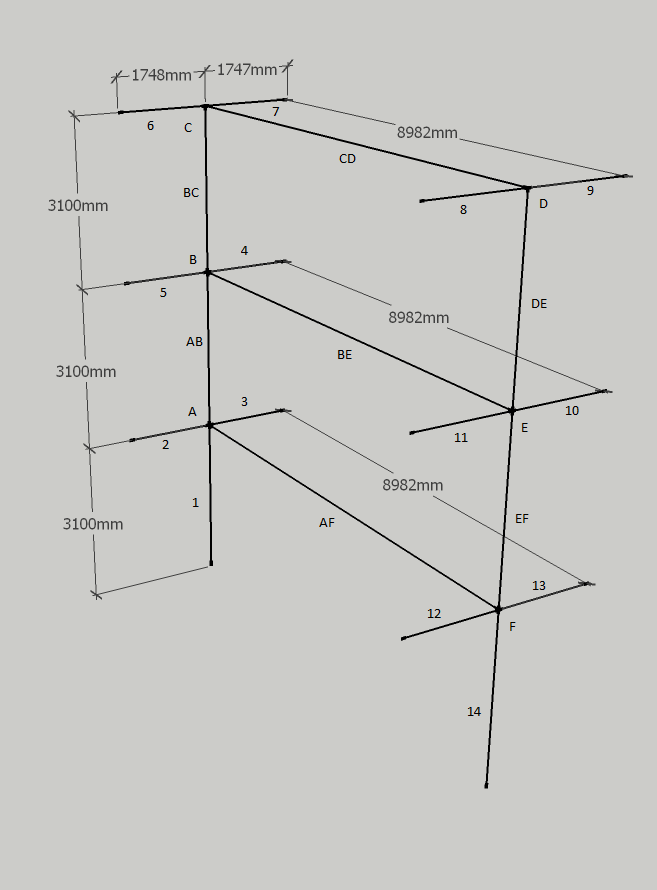
\includegraphics[width=0.7\textwidth]{billeder/Staaldimensioner_5}
	\caption{Viser en 3D model af rammens stållayout }
	\label{fig:EL1}
\end{figure}	
	
	Denne ramme bærer altså denne mængde af bygningen
\begin{figure}[H] 
	\centering
	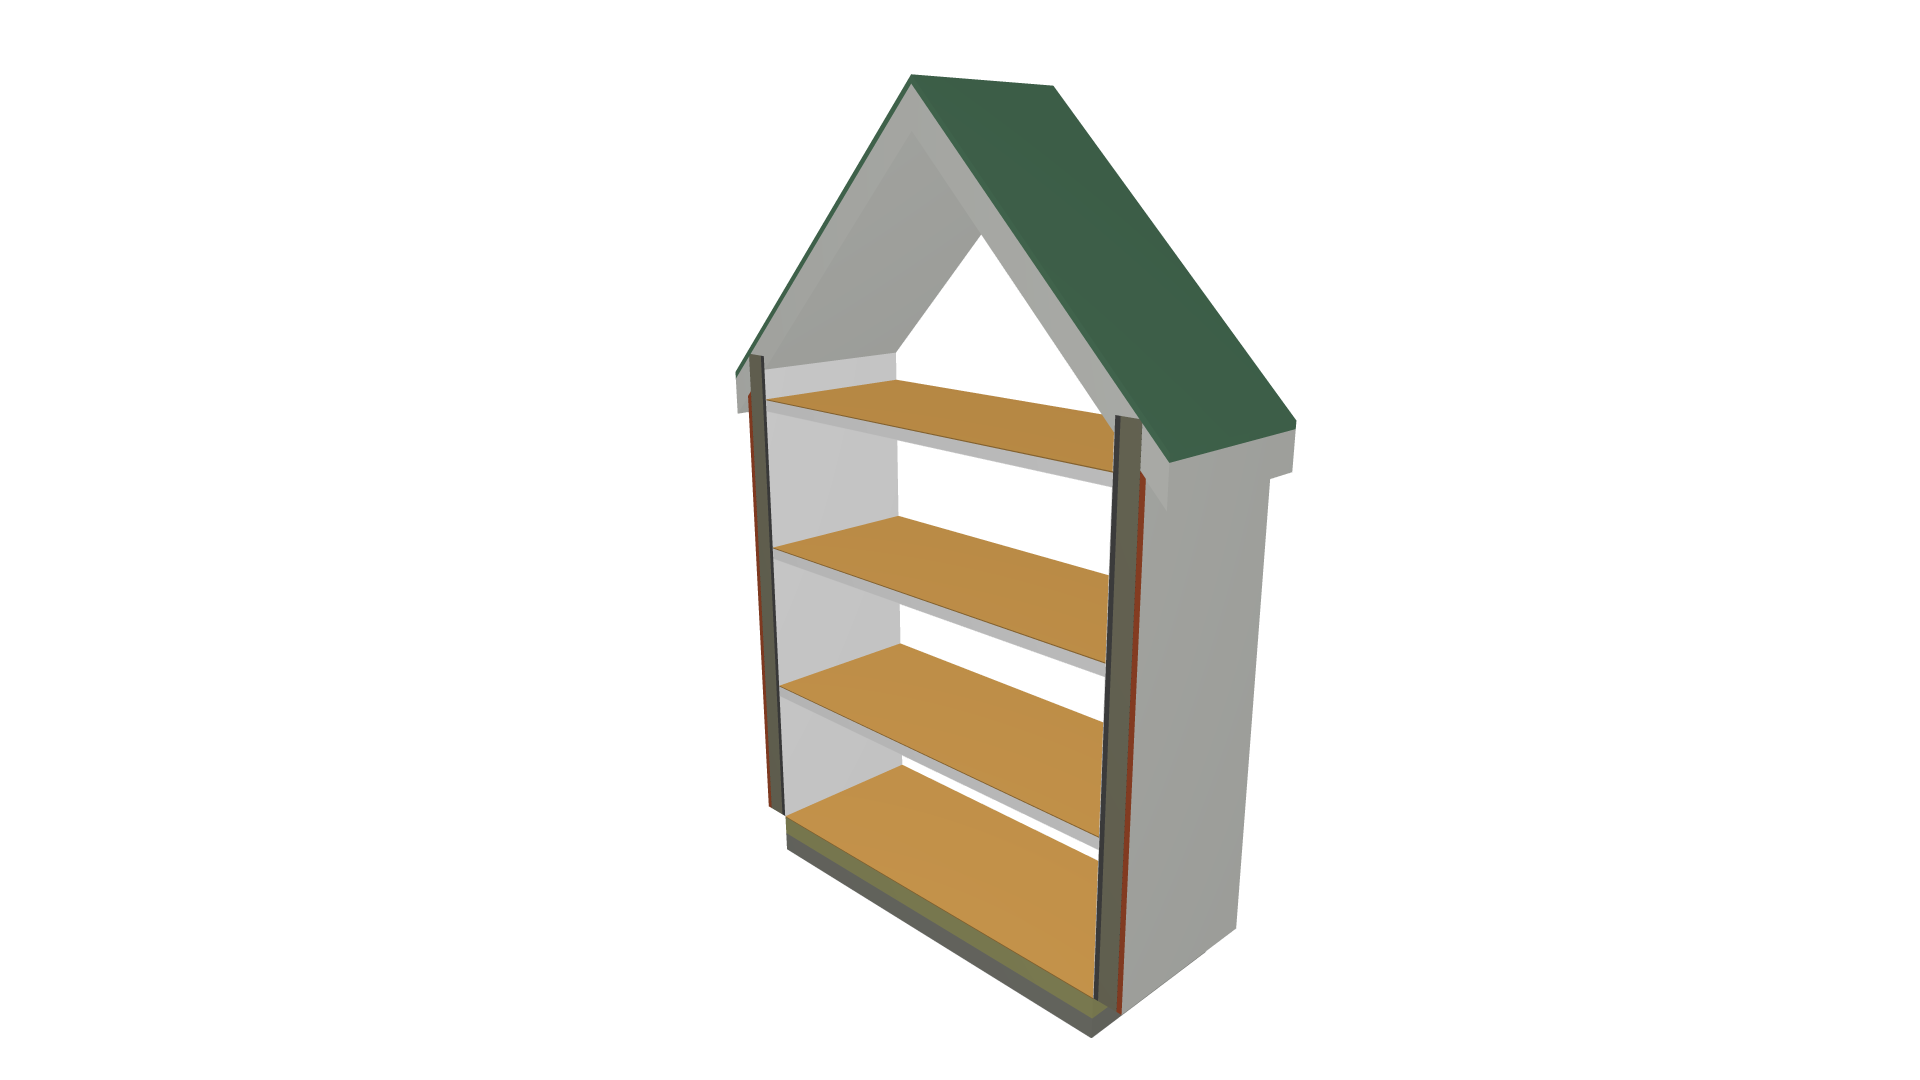
\includegraphics[width=1\textwidth]{billeder/Tvaersnit1}
	\caption{Viser en 3D model af de elementer, som stålrammen på Figur \ref{fig:EL1} bærer}
	\label{fig:EL2}
\end{figure}

I tabellen herunder ses ydervæggenes opbygning. Tallene er for den ene side af bygningen, altså det som halvdelen af rammen bærer.
\begin{table}[H]
	\centering
	\begin{tabular}{lll|l|ll|l|l}
		\cline{4-4} \cline{7-7}
		&                                                        &      & Mængde ($m^{3}$) &                             &      & Vægt (kg) &                             \\ \hline
		\multicolumn{1}{|l|}{}           & \multicolumn{1}{l|}{Densitet ($\dfrac{kg}{m^{3}}$)} & St.  & 1. sal                       & \multicolumn{1}{l|}{2. sal} & St.  & 1. sal    & \multicolumn{1}{l|}{2. sal} \\ \hline
		\multicolumn{1}{|l|}{Teglsten}   & \multicolumn{1}{l|}{1500}                              & 1,17 & 1,17                         & \multicolumn{1}{l|}{1,17}   & 1755 & 1755      & \multicolumn{1}{l|}{1755}   \\ \hline
		\multicolumn{1}{|l|}{Mineraluld} & \multicolumn{1}{l|}{115}                               & 4,33 & 4,33                         & \multicolumn{1}{l|}{4,33}   & 498  & 498       & \multicolumn{1}{l|}{498}    \\ \hline
		\multicolumn{1}{|l|}{Gips}       & \multicolumn{1}{l|}{900}                               & 0,13 & 0,13                         & \multicolumn{1}{l|}{0,13}   & 117  & 117       & \multicolumn{1}{l|}{117}    \\ \hline
		\multicolumn{1}{|l|}{SUM}        & \multicolumn{1}{l|}{}                                  & 5,63 & 5,63                         & \multicolumn{1}{l|}{5,63}   & 2371 & 2371      & \multicolumn{1}{l|}{2371}   \\ \hline
	\end{tabular}
	\caption{Viser densitet af de anvendte materialer, samt materialeforbruget og massen på de forskellige etager}
	\label{tabel:EL1}
\end{table}

I tabellen herunder ses gulvenes opbygning. Tallene er for den ene side af bygning, altså det som halvdelen af rammen bærer.
\begin{table}[H]
	\centering
	\begin{tabular}{lll|l|ll|l|l}
		\cline{4-4} \cline{7-7}
		&                                                        &       & Mængder ($ m^{3} $) &                            &      & Vægt (kg) &                             \\ \hline
		\multicolumn{1}{|l|}{}          & \multicolumn{1}{l|}{Densitet ($ \dfrac{kg}{m^{3}} $)} & St.   & 1. sal                        & \multicolumn{1}{l|}{2.sal} & St.  & 1. sal    & \multicolumn{1}{l|}{2. sal} \\ \hline
		\multicolumn{1}{|l|}{Træ}       & \multicolumn{1}{l|}{500}                               & 0,314 & 0,314                         & \multicolumn{1}{l|}{0,314} & 157  & 157       & \multicolumn{1}{l|}{157}    \\ \hline
		\multicolumn{1}{|l|}{Hul beton} & \multicolumn{1}{l|}{2000}                              & 3,45  & 3,45                          & \multicolumn{1}{l|}{3,45}  & 6906 & 6906      & \multicolumn{1}{l|}{6906}   \\ \hline
		\multicolumn{1}{|l|}{Gips}      & \multicolumn{1}{l|}{900}                               & 0,157 & 0,157                         & \multicolumn{1}{l|}{0,157} & 141  & 141       & \multicolumn{1}{l|}{141}    \\ \hline
		\multicolumn{1}{|l|}{SUM}       & \multicolumn{1}{l|}{}                                  & 3,92  & 3,92                          & \multicolumn{1}{l|}{3,92}  & 7204 & 7204      & \multicolumn{1}{l|}{7204}   \\ \hline
	\end{tabular}
	\caption{Viser densitet af de anvedte materialer, samt materialeforbruget og massen på de forskellige etager}
	\label{tabel:EL2}
\end{table}

\newpage
I tabellen herunder ses tagets opbygning. Tallene er for den ene side af taget, altså det som halvdelen af rammen bærer.
\begin{table}[H]
	\centering
	\begin{tabular}{l|l|l|l|}
		\cline{2-4}
		& Densitet ($ \dfrac{kg}{m^{3}} $) & Mængde ($ m^{3} $) & Vægt (kg) \\ \hline
		\multicolumn{1}{|l|}{Tagsten}    & 2000                              & 0,522                        & 1044      \\ \hline
		\multicolumn{1}{|l|}{Mineraluld} & 115                               & 26,1                         & 3003      \\ \hline
		\multicolumn{1}{|l|}{SUM}        &                                   & 26,6                         & 4047      \\ \hline
	\end{tabular}
	\caption{Viser densitet af de anvedte materialer, samt materialeforbruget og massen af taget}
	\label{tabel:EL3}
\end{table}

Eftersom det i udregningen af egenlasten ikke vides, hvilke stålprofiler der skal benyttes, bliver disse indsat som konstanter i udregningerne, hvorved man efterfølgende i styrkeberegningerne kan finde frem til hvilke typer, der er passende.

\begin{figure}[H] 
	\centering
	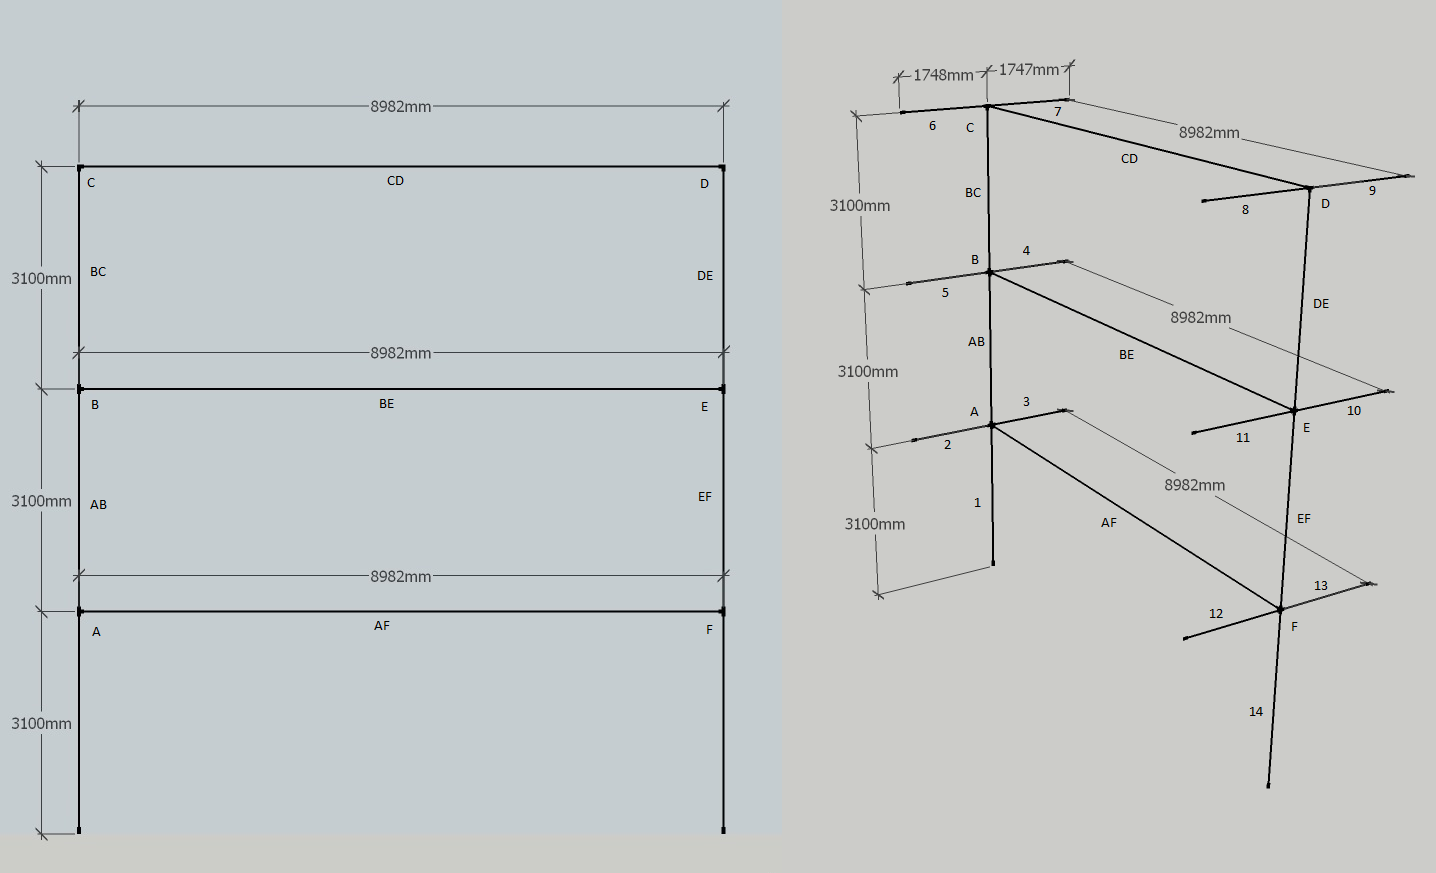
\includegraphics[width=1\textwidth]{billeder/Staaldimensioner_6}
	\caption{Viser en 3D model af stålrammen samt et tværsnitlayout}
	\label{fig:EL3}
\end{figure}

Beregnigner for egenlast i punkterne C og D. Konstruktionen er som nævnt symmetrisk omkring midten, så egenlasten bliver den samme i de to punkter. Denne tendens forsætter i de resterende punkter.
\newline
Tyngdeaccelerationen, g, sættes til $ 9,82\dfrac{N}{kg} $
\newline
Massen pr. meter for stålprofilerne betegnes, G, og måles i $ \dfrac{kg}{m} $. Størrelserne varierer og er ukendte. Så en stålbjælke eller søjle skrives eksempelvis som $ G_{CD} $.
\newline
Massen af taget, som den ene side af stålrammen bærer, angives som  $ m_{tag} $. Taget er ikke lavet af stål og kan derfor ikke ses på Figur \ref{fig:EL3}, men derimod på Figur \ref{fig:EL2}
\newline
Massen af gulvene, som den ene side af stålrammen bærer, angives som $ m_{gulv_{x}} $. Så et gulv der eksempelvis bæres af bjælken CD skrives $ m_{gulv_{CD}} $
\newline
\begin{center}
	$ P_{C/D}=m_{tag}\cdot g+G_{CD}\cdot g\cdot \dfrac{1}{2}\cdot 8,982m+m_{gulv_{CD}}\cdot g =110,5kN+k$
\end{center}

Beregninger for egenlast i punkterne B og E. 
\newline
Massen af murene angives som $ m_{mur_{x}} $. Så en mur der eksempelvis bæres af søjlen BC skrives $ m_{mur_{BC}} $.
\begin{center}
	$ P_{B/E}=P_{C/D}+G_{BE}\cdot g\cdot \dfrac{1}{2}\cdot 8,982m+m_{gulv_{BE}}\cdot g+m_{mur_{BC}}\cdot g+G_{BC}\cdot g\cdot 3,100m=204,5kN+k$
\end{center}

Beregninger for egenlast i punkterne A og F
\begin{center}
	$ P_{A/F}=P_{B/E}+G_{AF}\cdot g\cdot \dfrac{1}{2}\cdot 8,982m+m_{gulv_{AF}}\cdot g+m_{mur_{AB}}\cdot g+G_{AB}\cdot g\cdot 3,100m =298,5kN+k$
\end{center}

Beregninger for egenlasten i reaktionerne $ R_{1} $ og $ R_{2} $
\begin{center}
	$ P_{R_{1}/R_{2}}=P_{A/F}+m_{mur_{1/14}}\cdot g+G_{1}\cdot g\cdot \dfrac{1}{2}\cdot 3,100m=321,8kN+k$
\end{center}




%FIGUR REFERENCE
%på Figur \ref{fig:EL1} G

%DIS IS FOR PIC
%\begin{figure}[H] 
	%\centering
	%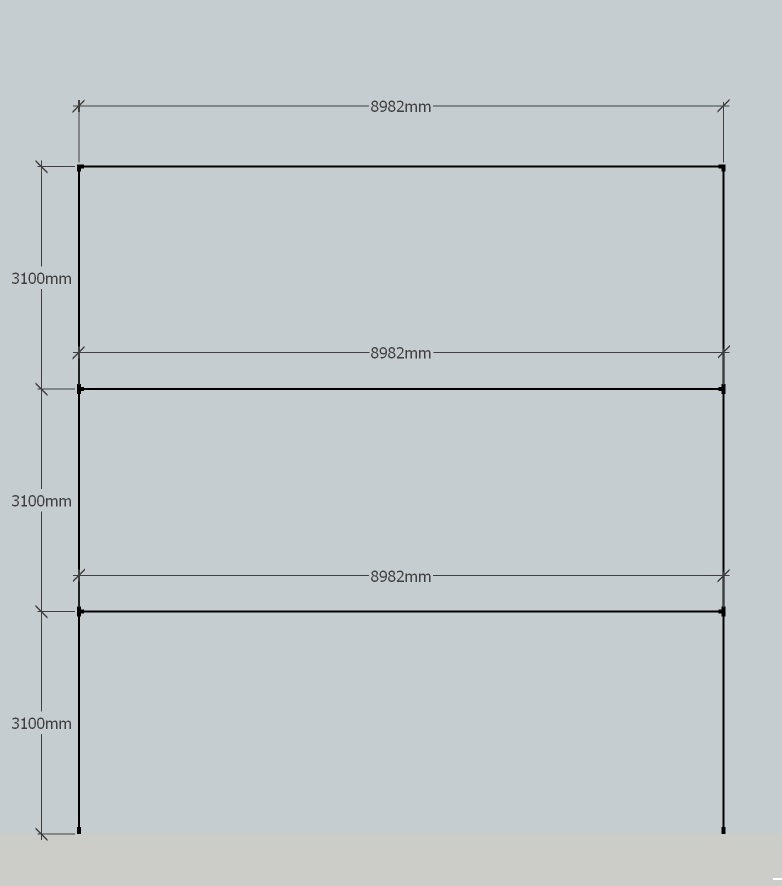
\includegraphics[width=0.5\textwidth]{billeder/Staaldimensioner}
	%\caption{Figuren viser }
	%\label{fig:EL1}
%\end{figure}

